\section{Hall sensor}
\subsection{What is a hall sensor?}
A Hall sensor is a transducer that varies its output voltage in response to changes in the magnetic field. It is often used to detect the presence or absence of a magnetic field and to measure the strength and polarity of the field. The Hall sensor operates on the principle of the Hall effect, where a voltage difference is created across a conductor when it is subjected to a magnetic field perpendicular to the current flow.\cite{9568879}

\subsection{What does a hall sensor do in our application?}
In our application, the Hall sensors play a crucial role in providing feedback on the rotor position of the Brushless Direct Current (BLDC) motor. The three Hall sensors are strategically placed around the motor to detect the magnetic field generated by the rotating magnets in the rotor. By monitoring the Hall sensor outputs, we can determine the rotor's position, allowing precise control of the motor and enabling closed-loop operation.\cite{7489411}

\subsection{Hardware}
For the hardware setup, initial attempts to read out values on the oscilloscope were unsuccessful. After consulting with Diego Zuidervliet\cite{zuidervliet2024}, it was suggested to add either a pull-up or pull-down resistor to stabilize the Hall sensor outputs.

A pull-up resistor connects the sensor output to a high voltage level, and a pull-down resistor connects it to a low voltage level. The purpose is to ensure a defined voltage level when the sensor is not actively providing a signal. In our case, we added a 10K ohm pull-up resistor to each Hall sensor output.

The wiring diagram, shown in \autoref{fig:hall_sensor_wiring_diagram}, depicts the connection of the pull-up resistors to the Hall sensor outputs. With this modification, we successfully plotted the Hall sensor information on the oscilloscope, providing stable and readable output.

\begin{figure}[H]
    \centering
    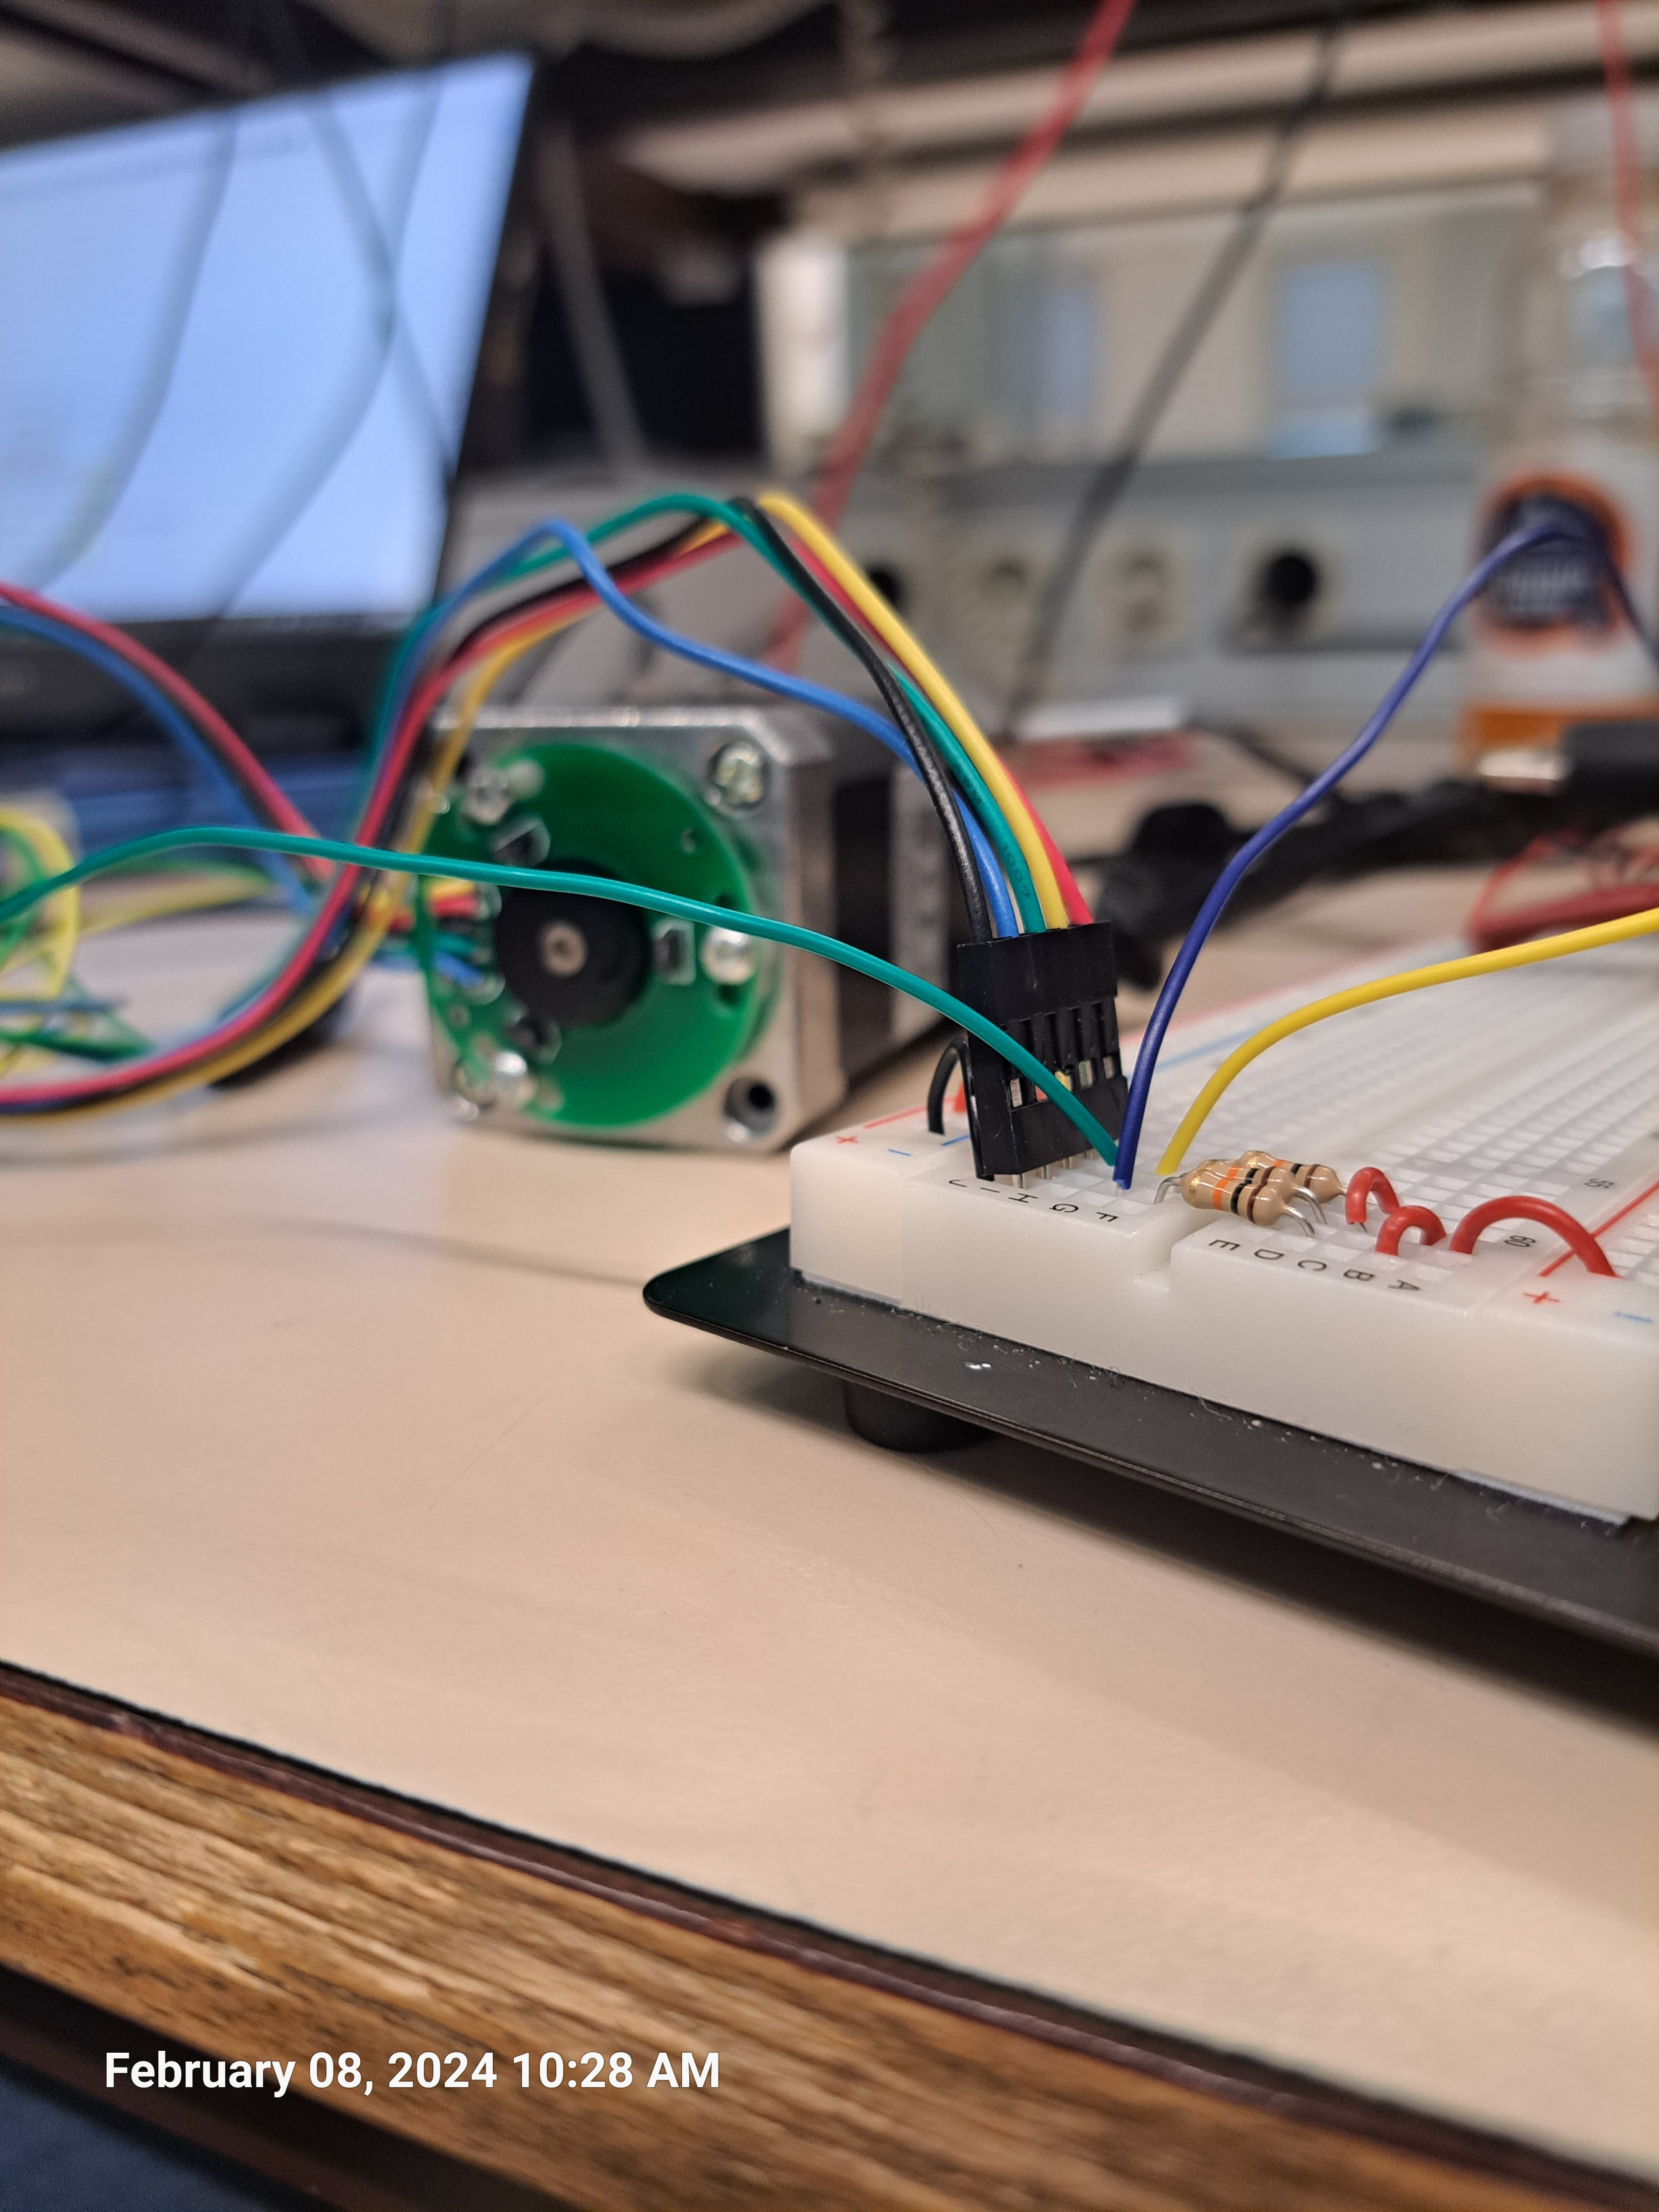
\includegraphics[width=0.3\textwidth]{img/Testing_Hallsensor_8-2-2024/Pictures/pull-up-resistor-breadboard-and-hall-sensor2.jpg}
    \caption{Wiring Diagram with Pull-up Resistors}
    \label{fig:hall_sensor_wiring_diagram}
\end{figure}

The circuit diagram, shown in \autoref{fig:hall_sensor_circuit_diagram}, illustrates the connection of the Hall sensors with the pull-up resistors.

\begin{figure}[H]
    \centering
    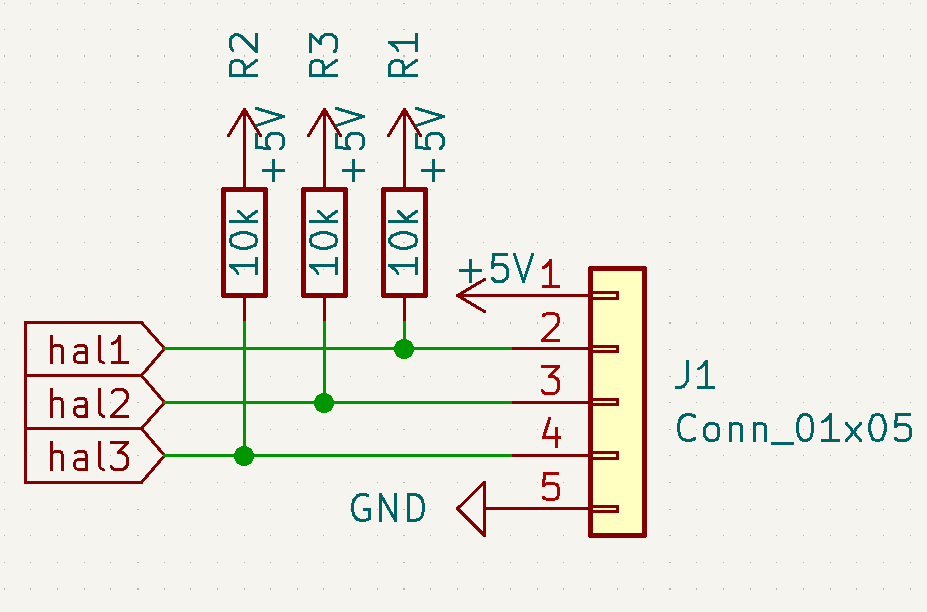
\includegraphics[width=0.45\textwidth]{img/Testing_Hallsensor_8-2-2024/Circuit/hall_sensor_circuit.png}
    \caption{Circuit Diagram with Pull-up Resistors}
    \label{fig:hall_sensor_circuit_diagram}
\end{figure}

Since we now understand the Hall sensor's function, its role in our application, and how to obtain stable readings, we can proceed with the software development.



\subsection{Software}




